\documentclass[12pt]{article}

\usepackage{sbc-template}

\usepackage{graphicx,url}

%\usepackage[brazil]{babel}   
%\usepackage[latin1]{inputenc}
\usepackage[utf8x]{inputenc}  

     
\sloppy

\title{Máquina de Turing Universal e sua Influência na \\ Arquitetura dos Computadores Modernos \\}

\author{Tiago Augusto Engel\inst{1}, Vanderlan Dupont de Oliveira\inst{1}}
\address{Acadêmicos de Ciência da Computação\\
Universidade Federal de Santa Maria -- UFSM
\email{\{tengel, voliveira\}@inf.ufsm.br}}


\begin{document} 

\maketitle
\begin{resumo} 
 Este artigo descreve a Máquina de Turing Universal. O objetivo é apresentar resumidamente o que é a máquina, quais as suas características e a sua influência na Arquitetura dos Computadores Modernos, a qual baseia-se nas idéias desenvolvidas por John Von Neumann.
\end{resumo}

\begin{abstract}
This paper describes de Universal Turing Machine. The goal is to summarize what is the machine, which are its features and its influence on the architecture of modern computers which is based on the ideas developed by Von Neumann.
\end{abstract}
     

\section{Introdução}

As primeiras idéias de computador surgiram com Alan Turing e sua idéia de “uma única máquina que pode ser usada para computar qualquer sequência computável”, depois as idéias dividiram-se em duas versões. Uma delas é britânica e foi batizada de Colossus, computador construído pela equipe de Turing no Bletchley Park para viabilizar a quebra de códigos de guerra Alemães que eram conhecidos como Códigos Enigma. A outra versão é Americana e começa com a construção do ENIAC na Universidade de Pensilvânia em 1943, e continua através da industrialização dessa tecnologia através de indústrias como Univac e IBM, que foram pioneiras na criação de um mundo o qual o computador se tornou ferramenta indispensável.

Este artigo é dividido em duas seções principais. A seção dois trata de Alan Turing e sua máquina. A terceira seção trata da arquitetura de Von Neumann  e como ela se relaciona com o modelo proposto por Turing.

\section{Máquina de Turing}

Alan Turing ousou perguntar se uma máquina pode pensar. Suas contribuições para entender e responder à essa e outras questões desafiam classificações convencionais. No final do século XX, o conceito de máquina de Turing, criado em 1936, figura não apenas na matemática e na ciência da computação, mas também na ciência cognitiva e na biologia teórica \cite{hodges1999}. Seu artigo \emph{Computing machinery and intelligence} \cite{Turing1950} no qual é descrito o assim chamando Teste de Turing, constitui um marco para a teoria da inteligência artificial. Turing desempenhou um papel decisivo no resultado da Segunda Guerra Mundial, produzindo sozinho um plano muito avançado para a construção e o uso de um computador eletrônico.

Em 1936 Turing escreveu um artigo entitulado \emph{On Computable Numbers, with an Application to the Entscheidungsproblem}~\cite{Turing1936} que descrevia uma máquina hipotética a qual ele chamou "Máquina Universal de Computação", a qual ficou conhecida como  "Máquina de Turing Universal". A máquina hipotética tinha um armazenamento infinito que continha instruções e dados. Esse artigo é considerado o mais importante de toda a história da computação. Uma Máquina de Turing Universal (MTU) é uma Máquina de Turing que consegue simular qualquer outra máquina de Turing a partir da descrição daquela máquina. Essencialmente, essa simulação é realizada lendo-se tanto a descrição da máquina a ser simulada quanto sua respectiva entrada representada pelo conteúdo de sua fita. 

\begin{figure}[!ht]
\centering
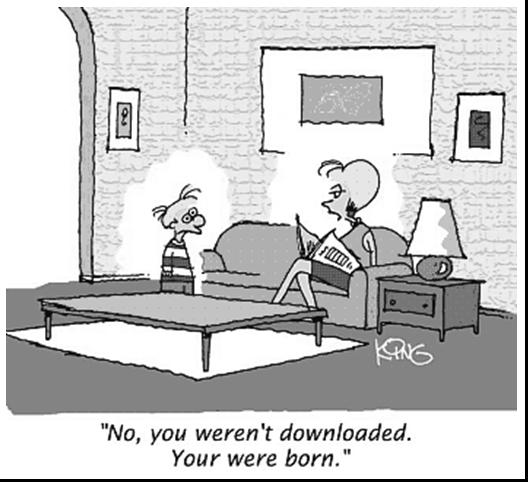
\includegraphics[width=.5\textwidth]{fig1.jpg}
\caption{Desenho esquemático de uma Máquina de Turing}
\label{fig:exampleFig1}
\end{figure}

Este modelo é considerado por alguns, segundo ~\cite{davis2001} como a origem do Computador com Programa Armazenado, usado por John von Neumann, denominado Arquitetura de Von Neumann. Ele se familiarizou com o trabalho de Turing que era professor visitante em Cambridge no ano de 1935. Se Neumann sabia do artigo de Turing de 1936 naquela época não é claro.

Naquela época, os computadores de guerra eram programados reconstruindo-se a maquina para realizar uma tarefa diferente. Por exemplo, o computador ENIAC tomou três semanas para poder desempenhar uma tarefa diferente. A nova idéia era de que não somente os dados deveriam ser guardados em memória, mas o programa que processa aquele dado também deveria ser armazenado na mesma memória. Essa idéia significava que um computador constuído com essa arquitetura seria muito mais fácil de programar. Efetivamente, o programa em si era tratado como dado.

\section{ Arquitetura de Von Neumann}

A Máquina de Turing foi aprimorada por Neumann em uma arquitetura de computadores que fundamenta os computadores construídos até hoje. Assim, a Arquitetura de Von Neumann, como é conhecida, é uma arquitetura de computador que se caracteriza pela possibilidade de uma máquina digital armazenar seus programas no mesmo espaço de memória que os dados, podendo assim manipular tais programas.

Essa nova arquitetura de Programa Armazenado foi comunmente conhecida pelo Arquitetura de von Neumann. Os fundamentos de seu trabalho foram descritas no artigo chamado \emph{First Draft of a Report on the EDVAC} em tradução literal seria "Primeiros Rascunhos de um Relatório no EDVAC". O mesmo foi escrito na primavera de 1945 e distribuída para o pessoal da Moore Escola de Engenharia. O artigo apresentou a primeira descrição escrita do conceito de programa armazenado e explicou como o programa armazenado processa informação.
O relatório organizou o computador em quatro partes principais: A Unidade Central de Aritmética, Unidade Central de Controle, a Memória e os dispositivos de entrada e saída.

A Unidade de Lógica era responsável por efetuar as quatro operações básicas da aritmética. A Unidade de Controle oferecia a sequência apropriada de operações e fazia as unidades individuais agirem juntas para carregar uma tarefa específica programada o sistema. A Memória deveria armazenar dados numéricos e instruções codificadas numericamente. As unidade de Entrada e Saída servem de interface de interação para os usuários do computador.
Um diagrama básico da organização de Neumann pode ser visto na figura \ref{fig:exampleFig2}:


\begin{figure}[!ht]
\centering
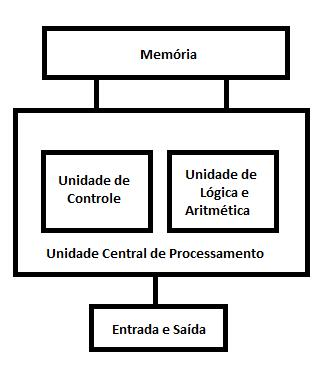
\includegraphics[width=.3\textwidth]{fig2.jpg}
\caption{Diagrama esquemático da arquitetura de Von Neumann.}
\label{fig:exampleFig2}
\end{figure}

Essa arquitetura é utilizada ainda hoje nos computadores. As diversas unidades são conectadas por um barramento (bus) de dados. A memória de acesso randômico remete à fita da máquina de turing, ela é randômica no sentido de que qualquer posição de memória tem o mesmo tempo de acesso.

A partir do conceito de manipulação de endereços de memória surgiram os conceitos das primeiras linguagens de programação Imperativas. Isso significa que efetuar uma computação implicaria em alterar endereços de memória para chegar em algum resultado. Esse conceito é utilizado nas linguagens mais utilizadas hoje em dia, ele é possível graças à arquitetura desenvolvida.


\section{Conclusão}
Turing introduziu seu modelo abstrato de máquina na sua primeira grande publicação \emph{On Computable Numbers, with an Application to the Entscheidungsproblem}~\cite{Turing1936}.  Esse artigo foi pioneiro da idéia essencial do computador moderno. O conceito de controlar as operações de uma máquina através de instruções codificadas armazenadas  na memória se aplica em toda a computação atual.

Não é citada diretamente por Neumann em seu primeiro trabalho a respeito do trabalho que tinha sido desenvolvido anteriormente por Turing. Alguns estudiosos do assunto como ~\cite{davis2001} acreditam que Neumann sabia sobre o que Turing estava desenvolvendo. O fato é que essas duas mentes são consideradas as criadoras da Computação.

\bibliographystyle{sbc}
\bibliography{ref}

\end{document}
